% !TEX program = pdflatex
\documentclass[12pt]{article}
\usepackage[reqno]{amsmath}
\usepackage{amssymb,amsthm,graphicx,verbatim,url,verbatim,longtable,vmargin, accents,bbm,times,subfig,dcolumn,booktabs,setspace,soul,latexsym,wasysym,titling,enumitem,longtable,booktabs,xr,caption}
\externaldocument{acc-supp}
\allowdisplaybreaks
% \usepackage{showkeys}

\usepackage[export]{adjustbox}
\usepackage[dvipsnames,usenames]{xcolor}
\definecolor{spot}{rgb}{0.6,0,0}

\usepackage{tikz}\usetikzlibrary{tikzmark,arrows,calc,arrows.meta}
\usepackage[T1]{fontenc}\usepackage[encapsulated]{CJK}\usepackage[utf8]{inputenc}

\newcommand{\icirc}{%
  
\begin{tikzpicture}[baseline=(char.base)]
    \node[shape=circle, fill=lightgray, font=\normalsize, inner sep=1pt, minimum size=1em] (char) {\textcolor{white}{i}};
  \end{tikzpicture}%
}

\usepackage[natbib=true,uniquename=false,minbibnames=1,maxbibnames=99,maxcitenames=1,maxcitenames=3,backend=biber,ibidtracker=false,style=authoryear]{biblatex}
\addbibresource[location=remote]{https://raw.githubusercontent.com/iqss-research/gkbibtex/master/gk.bib}
\addbibresource[location=remote]{https://raw.githubusercontent.com/iqss-research/gkbibtex/master/gkpubs.bib}
\setcounter{biburllcpenalty}{7000}\setcounter{biburlucpenalty}{8000}

\usepackage[all]{xy}
\setpapersize{USletter} \topmargin=0in
\newcolumntype{.}{D{.}{.}{-1}}\newcolumntype{d}[1]{D{.}{.}{#1}}
\graphicspath{{./figs/}}
\renewcommand{\topfraction}{0.85} \renewcommand{\textfraction}{0.1}
\renewcommand{\floatpagefraction}{0.75} % keep < \topfraction
\newcommand{\cntext}[1]{\begin{CJK}{UTF8}{gbsn}#1\end{CJK}}
\newcommand{\btVFill}{\vskip0pt plus 1filll}
\usepackage[titletoc,title]{appendix}
\newtheorem{proposition}{Proposition}
\DeclareMathOperator*{\argmax}{arg\,max}
\DeclareMathOperator*{\argmin}{arg\,min}
\newcommand{\mean}{\operatornamewithlimits{mean}}  
\newcommand{\Cov}{\text{Cov}}
\theoremstyle{definition}
\newcommand{\blind}{0} % 1=blind, 0=not blind
\newcommand{\titl}{Statistical Intuition Without Coding (or Teachers)}
\newcommand{\authr}{Natalie Ayers, Gary King, Zagreb Mukerjee, Dominic Skinnion}

\if1\blind
\title{\titl}
\renewcommand{\authr}{}
\fi
\usepackage[pdftex, bookmarksopen=true, bookmarksnumbered=true,
  pdfstartview=FitH, breaklinks=true, urlbordercolor={0 1 0},
  citebordercolor={0 0 1}, colorlinks=true, citecolor=spot, 
  linkcolor=spot, urlcolor=spot, pdfauthor={\authr},
  pdftitle={\titl}]{hyperref}

\if0\blind

\title{\titl\thanks{Our thanks to Kenneth Bollen, Aleksandra Conevska, Jamie Druckman, Danny Ebanks, Zach Elkins, Benjamin Goodrich, Connor Jerzak, David Kane, Thad Kousser, Adeline Lo, Thomas Pepinsky, Yotam Shmargad, Fred Oswald, and an anonymous reviewer through the Alexander and Diviya Magaro Peer Pre-Review Program for helpful comments. Our thanks to Evan Sarmiento, Rebecca Nichols, Mike Reekie, and Andrew Juraschek for help in product development.}}

\author{Natalie Ayers\thanks{Political Science Ph.D.\ student, Institute for Quantitative Social Science, Harvard University, Natalie-Ayers.github.io/home, NatalieAyers@g.harvard.edu}\and Gary King\thanks{Albert J.\ Weatherhead
III University Professor, Institute for Quantitative Social
Science, Harvard University; GaryKing.org, King@Harvard.edu.}\and Zagreb Mukerjee\thanks{Political Science Ph.D.\ student, Yale University, politicalscience.yale.edu/people/Zagreb-Mukerjee, Zagreb.Mukerjee@Yale.edu} \and Dominic Skinnion\thanks{Quantitative Social Science Researcher, Institute for Quantitative Social Science, Harvard University, Dominic\_Skinnion@g.harvard.edu, iq.harvard.edu/people/Dominic-Skinnion}}
\fi

\begin{document}
\maketitle\thispagestyle{empty}\setcounter{page}{0}
\btVFill
\vspace{-2\baselineskip}
\begin{abstract}
  \noindent Teaching political methodology classes typically requires a set of technical, instructor-led lectures on sophisticated statistical concepts (such as probability modeling, inference, and proper interpretation), followed by chances for students to iteratively adjust methodological specifications, parameters, and datasets so they can understand how each combination affects the results. Iteration is essential to learning complicated concepts, but until now has required simultaneous mastery of a statistical programming language (such as R), which makes learning both harder. Teaching R the semester before would make methods classes easier but also delay research experiences and demotivate our students eager to begin substantive research. We address both problems through a new type of interactive teaching tool that lets students iterate while learning the big conceptual picture and all its separate parts without having to simultaneously become programmers.  We make this tool available for use in classes now (via \href{https://2k1.iq.harvard.edu}{one click in a web browser}) and as an example of a new type of more friendly methods instruction for students and instructors alike.
  \\
  \newline
  \noindent Words: 2735
\end{abstract}
\btVFill
\clearpage
% \renewcommand{\contentsname}{Contents (page to be removed before publication)}
% \setcounter{tocdepth}{8}\tableofcontents\clearpage
\baselineskip=1.57\baselineskip

\section{Introduction}\label{s:intro}

Most new political science Ph.D.\ students have long since branched off from math and physics and are excited to be able to focus on their substantive interests in government and politics. Yet, upon arrival, many are surprised to learn that their first class will be in quantitative political methodology, and they now need to master a series of highly sophisticated technical concepts, such as the mathematical and statistical theories of uncertainty and inference. Because ``deferral of gratification'' pretty much defines the graduate school experience, most dutifully go along. But then they arrive in class, expecting to be taught these abstract concepts and are told that they must simultaneously learn the practical details of a statistical programming language --- so that they can learn (and implement) these abstract concepts, in order to begin to study what they came to graduate school for in the first place. 

Abstract statistical theory and practical programming tasks (including, e.g., understanding how maximum likelihood differs from probability theory and fixing that obscure bug in your code on line 57) are, of course, both essential to a career as an empirical political scientist. Statistical theory is the inferential foundation for social science research whereas programming enables students to learn by iterating between concept, statistical specification, data, and results, and later on to automate data wrangling and analysis. Although learning these two topics sequentially would be easier and more efficient, it can delay getting to substantively oriented research and thus demotivating to some. So instructors often teach both while also trying to give students the big picture of how research is justified, designed, and implemented all at the same time, often finding creative ways of using this material to motivate them \citep{williams2022teaching}. Judging from the dramatic changes in the literature over the last several decades, teachers of political methodology have succeeded spectacularly well in motivating students and making them better political scientists, but even with the best pedagogical strategies our classes do sometimes have the same problems as origami taught during swimming lessons.

In this paper, we propose a new approach to teaching political methodology that enables students to learn from iterating in this way following a lecture on difficult conceptual issues, without having to simultaneously learn programming (and thus with minimal distracting ``clutter''; \citealt{bailey2019teaching}). We aim to encourage that this approach be taken as new teaching innovations are developed in the future. We describe our ideas in principle in this paper and also provide an example that shows how it works in practice via software we developed called ``2K1-in-Silico: An Interactive Non-Textbook,'' which is available by clicking on \href{https://2k1.iq.harvard.edu}{2K1.iq.harvard.edu} (no downloads or installations required). Alternatively, you can download the app from our repository \href{https://github.com/iqss-research/2k1-in-silico}{github.com/iqss-research/2k1-in-silico} and install and use it offline, or try it in RStudio as a transition to learning to program. This is fully functioning software that we have extensively field tested in class after the instructor gives their usual full lecture on each part (thus helping to ``teach students to teach themselves''; \citealt{Schleutker2022}), but we offer it here primarily as an example of the kind of innovations in teaching and learning that future instructors might consider developing. Our software covers some of the most commonly taught difficult topics in political methodology classes, but obviously only a small subset of what could be taught. To bring our approach to other topics, we have made our software open source so other instructors can extend our software, or they follow the design principles described below and build new technologies from scratch.

2K1-in-Silco is named after the class for which it was originally designed, Government 2001, taught by Gary King. This is the first class in the Harvard University political science Ph.D.\ sequence and almost all graduate students in the department take it, along with students from related disciplines, professional schools, and nearby universities. 2K1-in-Silico can be used on its own, or by taking Government 2001 in residence at Harvard or online (through the Harvard Extension School).  Most of the materials for this class are also freely available to students and instructors elsewhere for use in their own classes. This includes all the lecture videos, the slides used in the lectures, the syllabus, the readings, and more; see the class website at \href{https://j.mp/G2001}{j.mp/G2001}. The lecture videos can be watched on your own on YouTube at \href{https://bit.ly/gov2001v}{bit.ly/gov2001v} or with others through \href{https://perusall.com}{Perusall.com}, a platform that allows students to help each other by annotating the videos and readings together and through other types of motivating interactions. Instructors teaching their own classes, or groups of students watching together, may create their own free Perusall class account by registering at \href{https://bit.ly/gov2001preg}{bit.ly/gov2001preg}, creating a course, and entering in ``copy code'' \textbf{PCDKPTWZ39}, which pulls in all these videos automatically.

\section{Approaches to Teaching and Learning}

We aim to enable political methodology instructors to follow the approach to teaching and learning that they have long espoused.  This approach is described in the ``Ideal Approach'' panel in Figure \ref{ov}.  We begin (as shown at the left of the top panel) with a carefully designed lecture on one of the many difficult topics in statistical theory or other sophisticated concepts in political methodology. For example, consider a class on maximum likelihood analysis covering the likelihood axiom, likelihood functions, how probability and likelihood differ, optimization, estimation, and properties of maximum likelihood estimators. (A more advanced class may even teach the general idea of extremum or M-estimators or connect maximum likelihood to related methods like non-linear least squares or the generalized method of moments.)
\begin{figure}[htb]
  \begin{center}
  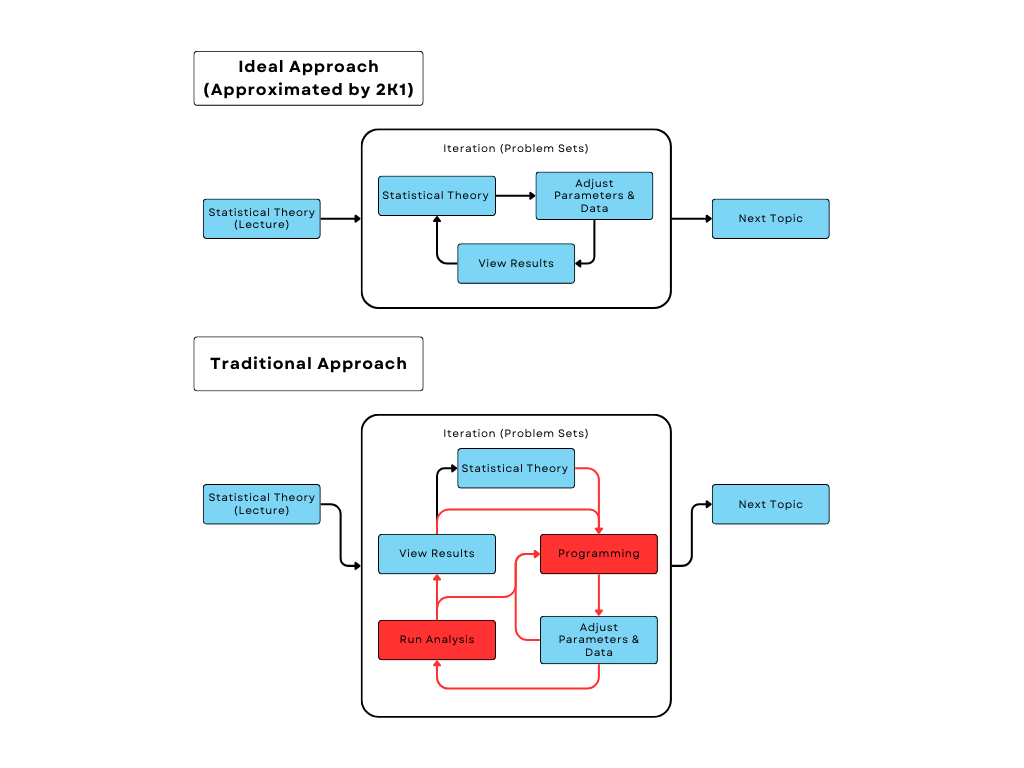
\includegraphics[width=\linewidth]{2}    
  \caption{Approaches to Teaching Methods}
  \end{center}
  \label{ov}
\end{figure}

Those of us who teach difficult topics like these learn a tremendous amount by giving lectures but no student understands all the information transmitted solely by listening. To learn, students must iterate --- they must use the knowledge in practice, try the concepts, and see how it all works. Thus, after lecture, we give the students problem sets, usually accompanied by sections and teaching assistants, where they can iterate by studying statistical theory from lecture, adjusting parameters and data, seeing how the results change, and going back to see how that corresponds to what they expect from the statistical theory (see the second item in the top panel of the figure).  After considerable effort iterating, successful students will have incorporated the knowledge that was transmitted in lecture into their long term understanding, and they can go on to the next topic, probably in lecture the next week (see third item in the top panel).

The goal of this approach to teaching is almost universal in political methodology classes, but the problem of requiring students to learn to program in the middle of iteration is something we all trip over while trying to implement.  To see this, consider the problem set that might be assigned after a class on maximum likelihood, consisting of a problem that can be solved with maximum likelihood estimation, perhaps using real replication data from a recent or prominent article. Students will be tasked with using this technique to develop an estimator, calculate estimates and standard errors, and perhaps confidence intervals or quantities on a scale of substantive interest rather than easy optimization.

The problem is that to realize the pedagogical value of this idealized approach, students have to be asked to learn the relevant programming tools, since most will be conducting numerical optimization for the first time.  We illustrate this in the second panel of Figure \ref{ov}, with the distracting but essential programming parts added in red. For example, in R, they may learn the use of the \verb|optim| function in order to maximize a log-likelihood. Given the challenges of numerical optimization, this will probably also require understanding of error handling via \verb|tryCatch| or related tools. If this comes relatively early in a class, this will also require a discussion of the role of functions in R, and the (often unintuitive) idea of a function as a first-class object that can be passed to other functions. 

Anecdotally, teaching assistants spend more than half of their office-hours on questions relating to the programming-specific aspects of the class. And frequently students who come into the class with programming experience spend considerable time helping the teaching staff by tutoring their classmates. In fact, the vast majority of complaints about political methodology classes across instructors we have talked with centers around programming, in classes that are not primarily about programming.

Of course, the learning objectives are logically sequential: First learn the programming, and then learn the methodology. But since student and instructor time is finite, these goals frequently end up competing. Even in the best case, when students have enough time to first learn the programming and then return to the statistics afterwards, the logical flow of the lesson is interrupted. After spending hours on debugging code that breaks when a Hessian is non-invertible, students often lose sight of the big picture: how maximum likelihood estimation does or doesn't correspond to inverting a matrix, and when it is a useful tool for political scientists --- especially since students may not have a complete understanding of that big picture until they've done some hands-on learning themselves. Spending so much time on technical minutiae while struggling to comprehend highly sophisticated theoretical concepts can be demotivating, if not demoralizing.

Instructors have addressed this problem in creative ways, such as by providing students with replication code that acts as a starting point for their own solutions. But, as many frustrated students of our classes will attest, running replication code can be a formidable technical challenge in itself, especially if you do not know precisely what the code is doing.

With our suggested direction (and with 2K1-in-Silico as an example), iteration can be much closer to the top panel in the figure.  Instead of first asking students to learn R, functions, optimization routines, and write a computer program, we can instead ask a series of discussion-style questions that can be answered with deep study using the 2k1 tool. How can we guess the bias of a coin from observing related flips? What does event count data look like when the underlying data generation process is Poisson-shaped? How does increasing the number of observations increase the curvature of the maximum-likelihood surface, and thus reduce the width of confidence intervals? How does the quadratic approximation to the log-likelihood work in practice with different datasets and modeling specifications?

The concepts political methodologists teach are some of the most highly sophisticated ideas they will find in graduate school. But we teach how to do research and the point of graduate school is to learn research, and so they cannot be skipped.  By enabling students to put aside programming, to switch from the bottom to the top panel of Figure \ref{ov}, students should be much better able to learn, understand, and incorporate the knowledge transmitted during lecture.

The new approach we recommend is thus not so new: It is the idealized approach we all try to use. The novelty we are suggesting is using modern technology to try to remove the distractions (the red from the bottom panel of Figure \ref{ov}) to enable instructors to do what they had intended all along, a topic to which we now turn.

\section{Interconnected Content}

Unlike connections that can often be found among substantive political science research topics, many parts of quantitative political methodology classes are closer to a singular whole and so best studied together. The difficulty is that any digestible, single class- or assignment-sized, piece of this whole is insufficient to convey the big picture. So we march forward, teach each part, and all the while ask students to trust us that the big picture, and fuller understanding, will come into focus over the semester. Because each part is best understood only after understanding all the other parts, students typically refer back to material learned earlier, or sometimes repeat the class or take different classes covering the same material.

2K1-in-Silico covers three interrelated topics that together form the centerpiece of much social science statistical modeling and analysis:
\begin{enumerate}\singlespacing
  \item \emph{Data generation processes}, using probability models;
  \item \emph{Inference}, using likelihood models \citep{King98}; and
  \item \emph{Quantities of interest}, using statistical simulation (see \citealt{KinTomWit00} and Clarify software for R or Stata; see \href{https://GaryKing.org/clarify}{GaryKing.org/clarify}).
  \end{enumerate}
Learning each of these sophisticated concepts is made much easier when iterating by adjusting parameters, model specifications, and datasets, and watching whether how the results change are compatible with your understanding of the statistical theory.

Probability enables us to randomly generate data from an assumed mathematical model (e.g., drawing a set of heads and tails from the model of a fair coin flip), whereas the goal of inference is the reverse: learning about features of a given model (such as whether the coin is fair) from a set of observed data (e.g., an observed string of heads and tails from 100 flips of a coin). Quantities of interest are calculated from statistical inferences, based on real data; numerous types of quantities can be computed, such as expected values, predicted values, and probabilities, for use in forecasts, descriptive and counterfactual estimation, or for other purposes
.
Probability, inference, and quantities of interest are mostly useful to political scientists with far more sophisticated models than coin flips, of course, allowing for explanatory variables and many possible different dependence structures, distributions, sample spaces, and mathematical formalisms.  2K1-in-Silico presently includes 18 different models, such as linear-normal regression, Poisson and negative binomial count models, exponential duration models, and binary and ordered probit and logit models. (Our software is open source, so anyone can add models if they wish, with some programming of course!)

Understanding one historical period or substantive topic studied by political scientists is usually helpful in studying another, but many topics in political methodology are much more interrelated.  The likelihood theory of inference is defined with probability densities. Computing quantities of interest can be done by simulation or analytic means to learn about the results of likelihood estimation or features of a probability distribution constructed from theory without data. Probability can be studied without the other two topics, but empirical political scientists have little interest in made-up models (or the data they can generate) without any necessary connection to the world we wish to study.

\section{Design Principles}

We suggest building tools for substantively oriented political scientists, and we built 2K1-in-Silico, by following four design principles.

First, the main idea is to provide the big picture while enabling students to zoom in and see any details they wish, with nothing omitted, and then zooming back out to understand the context. One of the reasons learning programming is valuable is because it enables us to get a feel for complicated statistical and mathematical objects (such as statistical models) too complicated to fit entirely in one human's working memory, usually by repeatedly running a program, changing its inputs, and seeing what happens to the outputs. We allow users to gain this intuition in 2K1-in-Silico by simple dropdown boxes and slider bars, and watching numerical results and graphics change dynamically and instantly, without any programming.

Second, the documentation for most statistical software packages does not include complete, mathematically precise descriptions of the methods and algorithms implemented, leaving instead only citations to the original scholarly source (sometimes with half-baked equations written in text, like DEPENDENT = alpha + beta1*INDEPENDENT, which usually conveys what is going on only to those who already know). For software users, however, determining whether the method implemented is identical to that in the textbook can then sometimes be difficult. In fact, anyone who writes computer code to implement a method knows that they typically do differ and for good reasons.

For one example, numerical optimization that involves a parameter that can only be positive, say a variance $\sigma^2$, can crash the program if it guesses zero or a negative value on the way to the optimum. Thus, a convenient numerical optimization trick is to reparameterize by defining $\sigma^2=e^\gamma$, and estimating $\gamma$. This is convenient because $\gamma$ can take on any finite value, and so we can optimize the function without constraints and without anything crashing, estimate $\gamma$, and then exponentiate the result. This works well also because $e^{\hat\gamma}$ is the same maximum likelihood estimate as if we had optimized the function directly. That's great but, in fact, the standard errors and full posterior distribution do change with this reparameterization and so replication, and complete understanding, requires knowing how the software is written. Thus, in 2K1-in-Silico, every time a user chooses a model, the full and precise mathematical formulation of the model implemented in the software automatically appears on the page (\LaTeX\ formatted).

Third, to make this tool work as well as possible without instructor intervention, we add next to every object on every page a \icirc\ symbol, enabling the user to request more \underline{i}nformation.  Clicking on any one of those symbols provides the needed information about an equation, dropdown box, statistical model, parameter, covariate, numerical result, dataset, or graphic. The information is presented in a little popup box without causing the user to lose context. In addition to all the \icirc\ symbols, there's a button to ask for a tutorial that will take you on a guided tour of the whole app if desired, which is designed for the most basic users without interfering with those with more advanced skills.

Finally, the program even tries to convey what numerical optimization algorithms do by letting the user guess at parameter values and see what the result looks like in terms of the distance from the maximum likelihood or what the uncertainty estimates look like. At every stage, the data are always available and on the screen, including data that could be generated by a probability model or to be used in making a statistical inference of some kind.

\section{What it Does}

Almost by definition, we cannot use the static presentation format of a paper to fully convey what our interactive tool does, and so feel free to click here \href{https://2k1.iq.harvard.edu}{2K1.iq.harvard.edu} and read along in order to see it in action as we explain it. In the app, you will find an overview page with three tabs across the top, corresponding to (1) data generation processes, (2) model inferences, and (3) quantities of inference, intended to be used in this order.  You can start with ``tutorial mode'' or instead skip that and see if the app is as intuitive enough without it, as intended. Either way, for any feature not immediately understandable, merely click on the corresponding \icirc\ to get an in-context, detailed explanation.

Begin by clicking on the data generation process (DGP) tab, and choosing a DGP to explore from the wide variety of examples listed. These include linear, normal, log-normal, Bernoulli, logit, probit, exponential, ordered logit and probit, and others. The mathematical form of the chosen probability model will instantly appear, along with slider bars for the user to set, indicating the parameter values and number of observations. This is followed by a dataset drawn from the model along with graphic visualizations in a variety of useful formats that automatically change depending on the type of data and model. All options, including the choice of the model, come with defaults, so you do not even need to make any choices if you prefer; however, you will gain intuition if you adjust the inputs and get a feel for how they and the model control the outputs.

To provide a better feel for the app if you have not yet clicked on the link, see Figure \ref{mockscreen} for a snapshot of the app's inference tab.  Along the top row, you can see the tabs that provide context.  Below that is the dataset the user created on the previous (DGP) page.  Although the data was generated by some model of the user's choice there, in the real world we do not know the DGP during inference. Thus, on this page we must choose the assumed distribution for the statistical model, which we can do from the dropdown box (on the top left, with ``Ordered Logit'' showing presently), along with the choice of one or more explanatory variables to include (with their own dropdown boxes, presently showing ``Normal B'' and ``Uniform A,'' with details about them documented in the gray \icirc\ symbol to its right).
\begin{figure}[p]
  %\null
  \vspace*{-1in} 
  \centering
  \begin{adjustbox}{center,valign=c}
    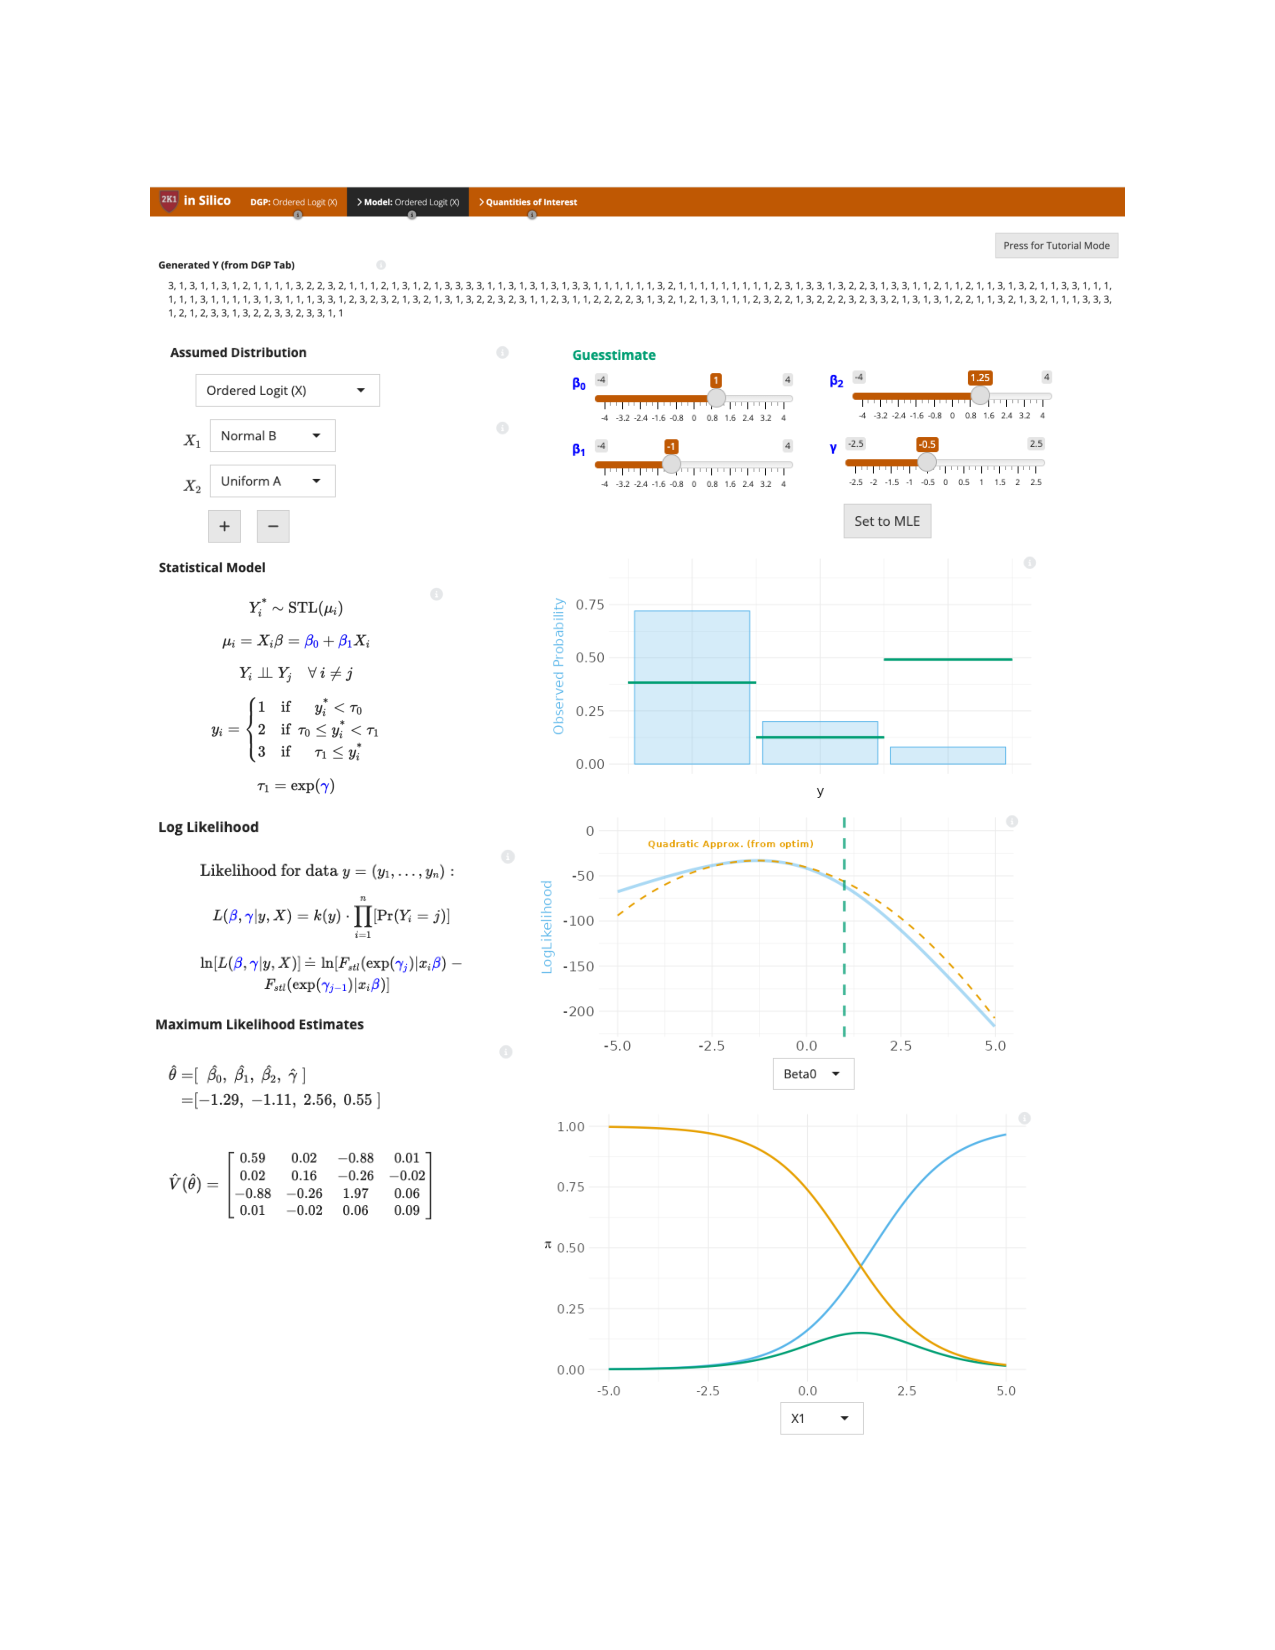
\includegraphics[width=1.5\textwidth]{mockscreen}
  \end{adjustbox}
  \vspace*{\fill} 
  \captionsetup{skip=-95pt}
  \caption{2K1-in-Silico: Model Inference tab (translated to a static figure)}
  \label{mockscreen}
\end{figure}

As soon as you choose an assumed statistical model, the mathematical form of the statistical model appears, followed by the complete mathematical form of the log-likelihood.  At the bottom left, the values of the maximum likelihood estimates and variance matrix appear, but to get a better feel for the maximization process, the slider bars at the top right allow the user to make a ``guesstimate'' of the values of each of the parameters (in blue, corresponding to the values in the math at the left). As the user adjusts these slider bars, the horizontal bars (in green, corresponding to the color of the word ``guesstimate'') in the graph below show how well they fit the empirical histogram of the data. The second graph plots the (profile) log-likelihood function for each parameter (chosen by the dropdown box below it), along with the best quadratic approximation to the log-likelihood which is used for calculating the standard errors.  The dashed green vertical line in this second plot shows how close the user's guesstimate is to the maximum of the log-likelihood function, and will move as you adjust the sliders.  The last graph on this page, which also instantly adjusts based on the slider bars, provides predicted values from the currently chosen model (in this case ordered logit, for each of the three outcome values that sum to one).  If you click on the ``Set to MLE'' button under the slider bars, the bars will adjust automatically to the maximum likelihood estimates, and the user will see the green horizontal bars on the first graph matching the histogram bars exactly, and all the other graphs adjusting automatically.

The last tab enables you to compute any of a variety of quantities of interest.  If you click on the tab, you will see at the top the maximum likelihood estimates and variance matrix from the inference tab. You can choose which quantity interests you and should be calculated.  Given that, the full mathematical details of the estimation and fundamental uncertainty appear, as these are needed for simulating quantities of interest. You can also select values of the explanatory variables via slider bars.  From all this information, 2K1-in-Silico automatically presents a set of colorful graphics to summarize the quantities you chose to compute, along with various types of uncertainty estimates.

At any time, you can go back to the main page to see the big picture, or any of the three tabs.

\section{Concluding Remarks}

We describe in this paper a tool designed to teach a large number of specific, interrelated topics.  We use this tool as an example of our main goal, to encourage thought about a new approach to teaching political methodology. Instead of requiring students to learn topics that happen to be convenient for existing technology, instructors and designers of teaching and learning tools ought to be able to modify the technology to meet students where they are and what they know. In this way, our students can learn the sophisticated concepts of political methodology better, be more motivated, and get up to speed faster. Students will likely still need to learn programming to do quantitative political science, but they can learn it when needed during their substantive research. This ``new'' approach is designed to use technology to achieve the idealized objectives of how most of us teach now.

In addition to trying 2K1-in-Silico or assigning it in class by clicking on \href{https://2k1.iq.harvard.edu}{2K1.iq.harvard.edu}, we hope readers will help us extend the tool to a wider variety of models, graphics, methods, and statistical concepts. We could even add additional tabs for understanding data, matching for causal inference, and imputation for missing data, among others. To do this, you will need to do some programming of course, but we use relatively straightforward R-Shiny technology, as recommended by \citet{Metzger2022}. All the code is open source and freely available at \href{https://github.com/iqss-research/2k1-in-silico}{github.com/iqss-research/2k1-in-silico}

And if the concepts you are trying to convey do not fit in an extension of our exsiting tool, we hope our design principles will be of use in building new tools that can be shared as widely.


\singlespace
\printbibliography
\end{document}


% Local Variables:
% TeX-engine: default
% TeX-master: t
% End:
